\documentclass[border=3pt,tikz]{standalone}
\usepackage[utf8]{vietnam}
\usetikzlibrary{calc,angles,intersections,shapes.geometric,arrows,decorations.markings,arrows.meta,patterns.meta,patterns}
\usepackage{tikz-3dplot,pgfplots}
\pgfplotsset{compat=1.15}
\usepgfplotslibrary{polar}
\usepackage{amsmath}
\begin{document}
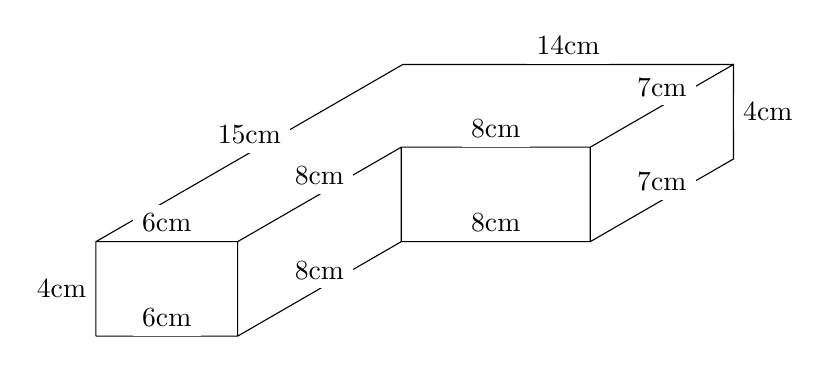
\begin{tikzpicture}[scale=.3]
	\def\a{6}
	\def\b{7}
	\def\c{8}
	\pgfmathsetmacro\d{int(\b+\c)}
	\pgfmathsetmacro\e{int(\a+\c)}
	\def\h{4}
	\def\g{30}
	\tikzset{every node/.style={midway,fill=white}}
	\draw
	(0:0)--++(0:\a)node[above]{\a cm}
	--++(\g:\c)node[above] {\c cm}
	--++(0:\c)node[above]{\c cm}
	--++(\g:\b)node[above]{\b cm}
	--++(90:\h)node[right]{\h cm}
	--++(\g-180:\b)node[above]{\b cm}
	--++(180:\c)node[above]{\c cm}
	--++(\g-180:\c)node[above]{\c cm}
	--++(180:\a)node[above]{\a cm}
	(0:0)--++(90:\h)node[left]{\h cm}
	--++(\g:\d)node[above]{\d cm}
	--++(0:\e)node[above]{\e cm}
	(0:\a)--++(90:\h)
	($(0:\a)+(\g:\c)$)--++(90:\h)
	($(0:\a+\c)+(\g:\c)$)--++(90:\h)
	;
\end{tikzpicture}
\end{document}